\documentclass[11pt,a4paper]{article}
%\usepackage{beamerarticle}

%\usefonttheme[onlymath]{serif}
\usepackage[ngerman]{babel}
\usepackage[utf8]{inputenc}
\usepackage[T1]{fontenc}
\usepackage{tikz}
\usetikzlibrary{positioning, arrows}
\usepackage{listings}
\usepackage{fancybox}
\usepackage{color}
\usepackage{hyperref}
\usepackage{fancyhdr}
\usepackage{extarrows}

\pagestyle{fancy}
\lhead{\today}
\author{Gruppe: SWT15-GKP}
\rhead{Author: KV}
\chead{Gruppe: SWT15-GKP}
%\cfoot{center of the footer!}
\renewcommand{\headrulewidth}{0.8pt}
%\renewcommand{\footrulewidth}{0.4pt}
\title{Universität Leipzig - Softwaretechnik Praktikum 2014/2015 \\  Entwurfsbeschreibung \\ zum Projekt: Ein kartenbasiertes “Multiplayer”-Spiel}

\begin{document}
\maketitle


\tableofcontents

\clearpage

\section{Allgemeines}
Im Rahmen des SWT-Praktikums wird ein kartenbasiertes Multiplayerspiel entwickelt, das es ermöglicht, ein an das alte Pacman angelehnte Computerspiel auf einem realen Kartenausschnitt zu spielen. Die entstehenden Highscores werden dann zu den jeweiligen Karten gespeichert um sich mit anderen Spielern messen zu können.


\section{Produktübersicht}
Der Nutzer kann online über die Spiele-Website auf das Programm zugreifen.
%Dabei stehen dem Nutzer ein Suchfeld zum finden der gewünschten Spielumgebung zur Verfügung, es kann auch manuell durch Scrollen über die Karte ein Spielort ausgewählt werden, wobei nur Städte ab einer bestimmten Größe zugelassen sind, damit auf jeden Fall eine spielbare Karte erstellt werden kann und die Highscore vergelichbar bleibt. 
Der Spieler kann duch Scrollen über die Karte einen Spieleort auswählen. Es sind nur bestimmte Orte als Spielort zugelassen, um eine Vergleichbarkeit zu gewährleisten.
Hat man den Ort ausgewählt, wird das Spielfeld erzeugt und man kann ein neues Spiel beginnen. 
Man kann den Pucman nun mit Hilfe der Pfeiltasten steuern.
Ziel des Spiels ist es den Pucman über die Karte zu steuern und die Kekse die auf der Karte verteilt liegen zu fressen. 

An dieser Aufgabe wollen den Spieler Geister hindern, die sich auch über das Spielfeld bewegen und Pucman fressen können. Frisst ein Geist den Spieler so wird dieser auf den Startpunkt zurückgesetzt und die Anzahl seiner Leben wird um eins verringert.
Es gibt unterschiedliche Geister, die durch ihr aussehen unterschieden werden können und sich anhand verschiedener Logiken bewegen. 
Falls keine Leben mehr übrig sind, wird das Spiel beendet und die erreichte Highscore zusammen mit der Karten URI und dem Namen des Spielers abgespeichert.
Während des Spielens werden die Möglichkeiten zur Veränderung der Kartenansicht deaktiviert. 
Das Spielgeschehen ist durch einen Soundtrack unterlegt, der eine funktionale und inhaltliche Verbindung zwischen Bild und Ton generiert.
Desweiteren werden für das Spiel wichtige Informationen wie aktueller Highscore, die verbleibende Anzahl an Leben und die Möglichkeit direkt auf die Website des Spiels zugreifen zu können angezeigt.
\clearpage
\section{Grundsätzliche Struktur- und Entwurfsprinzipien}
Als grundsätzliche Programmiersprache haben wir uns für Java-Script entschieden. Wobei der Java-Scriptcode von einer HTML-Seite aufgerufen wird. Desweiteren benutzen wir Phaser als Gameframework.
Ein Teil der Software wurde mithilfe von Funktionen aus der Java-Script Bibliothek JQuery geschrieben, da diese eine intuitive Herangehensweise bietet und für uns verständlicher als klassiches JavaScript ist.
Die von uns umgesetzte Web-Anwendung basiert auf einer Client-Server Architektur. Wir arbeiten mit einem HTML-Server auf dem die Daten liegen, die vom Client abgefragt und an diesen übertragen werden. Diese Daten beinhalten auch den Gameblock, der dann vom Client ausgeführt wird. Außerdem gibt es noch ein Map-Module, welches das Level aus den Geo-Daten erstellt, die mithilfe der Overpass API von OpenStreetMaps bezogen werden. Dazu kommt das Highscore-Module, welches für die Verwaltung der Highscores verantwortlich ist.
Desweiteren kommt noch ein Datenserver hinzu, der die Highscores unter Verwendung eines Tripplestores speichert.\\
\begin{figure}[htb]
  \centering
  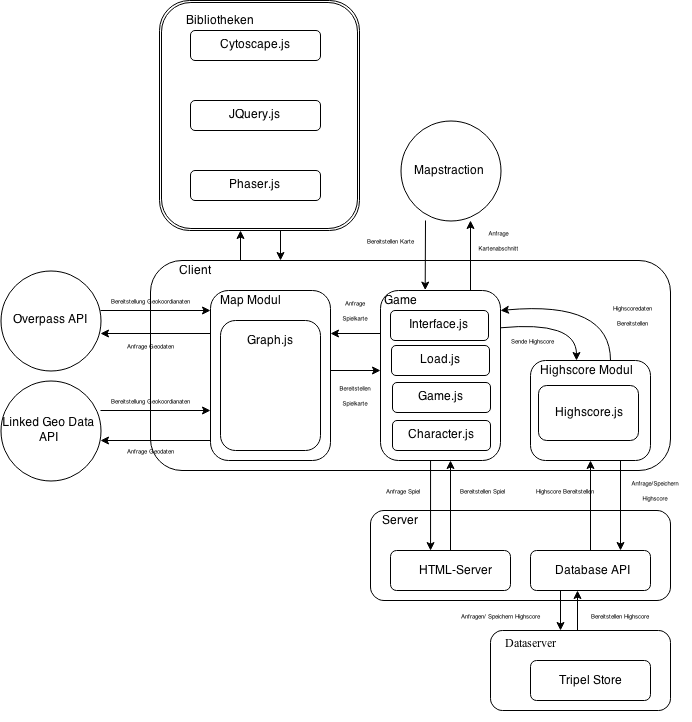
\includegraphics[scale=0.6]{dia_2.png}
\caption{Architekur}
  \label{arch}
\end{figure} 



\section{Struktur- und Entwurfsprinzipien der einzelnen Pakete}
\subsection{Server} Vom Server werden die benötigten Spieldateien zur Verfügung gestellt und automatisch geladen. Desweiteren werden Highscoreanfragen und Manipulationen zwischen dem Dataserver und dem Client verarbeitet und anschließend weitergeleitet.

\subsection{Client}
\subsubsection{Map-Modul}
%Die Linked GeoData API extrahiert aus OpenStreetMap die Geo-Daten für das Erstellen der Hintergrundkarte in Abhänigkeit vom gewählten Ort.\\

Die Overpass API extrahiert die Geo-Daten aus OpenStreetMap, die zum Hervorheben der benutzbaren Straßenzüge und zur Erstellung des Levels benutzt werden.\\
Die Datei \textbf{Graph.js} sorgt dafür, dass aus den Geo-Daten von OpenSteetMap weiterverarbeitet werden.
Die Erstellung des Spielgraphen ist in dieser Software, der aufwendigste Teil. \\
Durch eine Vorselektierung durch eine angepasste Query für die Overpass API werden die ersten Straßenzüge entfernt, wenn diese bestimmte Kriterien erfüllen, so wurden z.B. Fußwege, Fahhradwege, aber auch Treppen entfernt, die Herangehensweise dieser Anfrage war \glqq so wenig wie möglich, so viel wie nötig\grqq, das führt unter anderem dazu, dass die erstellten Graphen nicht zu groß werden, da wir ansonsten Probleme mit der Komplexität bekommen hätten. Es werden nur Straßen berücksichtigt, die in dem sichtbaren Bereich des Browser-Fensters liegen.\\
Die Anfrage liefert als Rückgabe eine Datei im GeoJson Format, welche wir mittels einem Parser durchlaufen und die relevanten Informationen in einen Graphen der Cytoscape Bibliothek übergeben, wir haben also nun einen Graphen im klassischen Sinne, Knoten, mit Geo-Koordinaten, und Kanten zwischen den Knoten. \\
Als nächsten Schritt haben wir die Koordinaten in Pixel auf dem Bildschirm umgewandelt.
In einer Iteration über alle Knoten werden nun Sackgassen gelöscht, da diese für uns unbrauchbar sind.
Wir haben auch Straßen aus dem Graphen entfernt, die in einer Kreuzung mit mehr als fünf Straßen münden. Wir wollen nicht zufallsgesteuert eine Straße auswählen müssen, wenn die Spielfigur an einer Sternkreuzung steht und zwei Straßen in die selbe Himmelsrichtung führen. \\
Da wir am jetzigen Zeitpunkt eventuell mehrere Graphen duch die Selektion der Straßenzüge erhalten haben, lassen wir einen Algorithmus über den Graphen laufen, der uns den größten zusammenhängenden Teilgraphen ausgibt. 
Als letzten Schritt müssen wir nun noch die Karte für uns spielbar machen, wir haben eine Knoten- und eine Kantenliste, um eine flüssige Bewegung zu gewährleisten, brauchen wir aber Pixel in bestimmten Abständen.
Es wird eine Interpolation gestartet, die zwischen den Knoten des Graphens die fehlenden Pixel setzt, s.d. die Spielfigur, sich über ein Netzt aus Pixeln bewegen kann, die eine bestimmte Dichte ausweisen. 
\subsubsection{Game-Modul}
Der Gameblock wird an das Model-View-Controller Prinzip angelehnt, welches durch die Nutzung von Phaser umgesetzt wird. 
Phaser übernimmt für uns die Eingabe und Ausgabeverarbeitung und stellt den Gameloop zur Verfügung, dies ist eine Schleife, die währen des Spielablaufs immer wieder durchlaufen wird.
Dabei werden im wesentlichen zwei Dinge ausgeführt:
Die Update-Methode, enthält: Tastatur- und Mauseingabe, Bewegung, Kollisionserkennung, ... \\
Die Render-Methode, enthält: Anzeige aller Sprites an den neuen Positionen, Hintergrund animieren, ... \\
Die Game Loop wird abgebrochen, wenn das Spiel beendet wird.
\par\bigskip
{\flushleft \textbf{Interface.js}} \\
In diesem Modul wird die Schnittstelle zum Benutzer definiert.
So werden hier z.B. Knöpfe und Anzeigen, die dem Benutzer Informationen über den aktuellen Spielstand liefern, bzw. diese Abrufbar machen erstellt.
Die Schnittstelle ist der Teil eines Systems, welcher der Kommunikation dient. \par\bigskip
{\flushleft \textbf{Load.js}} \\
Zeigt einen neuen Ladescreen, während die Karte lädt. \par\bigskip
{\flushleft \textbf{Game.js}} \\
Stellt den Gameloop dar. \par\bigskip
{\flushleft\textbf{Character.js}} \\
In diesem Modul wird die Spielfigur, also der Pucman definiert.

\subsubsection{Highscore-Modul}
Das Highscore Module verwaltet die Highscores der Spieler, d.h. es stellt Anfragen an den Server zum Triplestore und kann sie über den Server auch abfragen, falls sie im Spiel angezeigt werden sollen.
Die Highscores werden in einem Tripelstore gespeichert, welche mithilfe von SPARQL Queries abgefragt werden, bzw. durch  SPARQL Update Methoden in die Datenbank eingepflegt werden.
\subsection{Bibliotheken}
{\flushleft \textbf{Cytoscape.js}} \\
Diese Bibliothek wird von dem Map Modul benötigt um die Graphalgorithmen auszuführen. In der Bibiothek sind bereits viele Algorithmen enthalten.
{\flushleft \textbf{JQuery.js}} \\
Diese Bibliothek vereinfacht den Umgang mit verschiedenen Problem die auftraten.
{\flushleft \textbf{Phaser.js}} \\
Wie betreits erwähnt stellt Phaser als Gameframework einen sehr wichtigen Teil unseres Projektes dar, die Bibliothek stellt alle Funktionen zur Verfügung die man als Spieleentwickler benötigt um einen flüssigen Spielefluß, eine Eingabe- und Ausgabeverarbeitung etc. 
zu haben. 
\section{Datenmodell}

Siehe Abbildung \ref{arch}.\bigskip

Beschreibung zu Abbildung \ref{arch}: \\
$A \xlongrightarrow{\text{Datenfluß}} B $ beschreibt den Datenfluss von A nach B, wobei A und B Module der Software sind.


\section{Testkonzept}
Am Ende des Sprints wird die aktuelle Version der Software auf den Webserver geladen. Diese wird anhand eines \href{https://github.com/GKP15/pucman/wiki/Test-workflow}{Test-Workflows} geprüft. Dabei werden die angegebenen Eingaben getätigt und die Reaktion der Software mit der erwarteten Ausgabe verglichen. Sollten dabei Abweichungen auftreten, gilt der Test als nicht bestanden.

\section{Glossar}
Das Glossar wurde überarbeitet und als externes Dokument angefügt.
\end{document}